\documentclass[a4paper,landscape]{article}
\usepackage[margin=6mm]{geometry}
\usepackage[T1]{fontenc}
\usepackage{helvet}
\renewcommand{\familydefault}{\sfdefault}
\usepackage{microtype}
\usepackage{array,booktabs,tabularx,amssymb,colortbl}
\usepackage{xcolor}
\usepackage{tikz}
\usetikzlibrary{arrows.meta,positioning}
\usepackage[most]{tcolorbox}
\usepackage{enumitem}
\usepackage{hyperref}
\pagestyle{empty}
\setlength{\parindent}{0pt}
\setlength{\parskip}{1pt}
\setlist[itemize]{leftmargin=3mm,itemsep=0.2pt,topsep=0.3pt,parsep=0pt}
\setlist[enumerate]{leftmargin=3.6mm,itemsep=0.2pt,topsep=0.3pt,parsep=0pt}

\definecolor{VMTeal}{HTML}{006C78}
\definecolor{VMDark}{HTML}{143C50}
\definecolor{VMLight}{HTML}{EAF5F5}
\definecolor{VMGold}{HTML}{C98314}
\definecolor{VMGreen}{HTML}{1F8A55}
\definecolor{VMGray}{HTML}{F3F5F6}
\definecolor{VMRed}{HTML}{A33B36}
\hypersetup{colorlinks=true,urlcolor=VMTeal,linkcolor=VMTeal}

\newtcolorbox{vmBox}[2][]{
  enhanced,
  colback=white,
  colframe=VMTeal,
  boxrule=0.5pt,
  arc=1.5mm,
  left=1.7mm,right=1.7mm,top=1.3mm,bottom=1.2mm,
  title={#2},
  coltitle=VMDark,
  fonttitle=\bfseries\fontsize{8.5}{9.2}\selectfont,
  attach boxed title to top left={xshift=1.4mm,yshift=-1.7mm},
  boxed title style={colback=white,colframe=white,boxrule=0pt,left=0.4mm,right=0.4mm},
  before skip=0pt,after skip=0pt,
  #1
}

\newcommand{\yes}{\textcolor{VMGreen}{\bfseries\checkmark}}
\newcommand{\partmark}{\textcolor{VMGold}{\bfseries$\triangle$}}
\newcommand{\no}{\textcolor{VMRed}{\bfseries--}}
\newcommand{\source}[2]{\textsuperscript{\href{#1}{[#2]}}}

\begin{document}
\fontsize{7.15}{8.1}\selectfont

% Header
\begin{minipage}[t]{0.72\textwidth}
{\fontsize{18}{19.5}\selectfont\bfseries\color{VMDark}VentureMath}\hspace{1.6mm}
{\fontsize{10.4}{11.4}\selectfont\bfseries\color{VMTeal}Uncertainty-Certified AI Compiler for Minimum-Viable Hardware Digital Twins}

{\fontsize{8.0}{8.9}\selectfont\color{black!78}
Turning venture intent, component documentation, and a minimal set of physical measurements into a traceable, calibrated, decision-ready simulation before a full hardware build.}
\end{minipage}
\hfill
\begin{minipage}[t]{0.255\textwidth}
\raggedleft
\colorbox{VMLight}{\parbox{0.95\linewidth}{\centering\bfseries\color{VMDark}Concept One-Pager --- Working Draft\\[-1pt]\normalfont\fontsize{6.7}{7.4}\selectfont Internal discussion and collaborator outreach}}
\end{minipage}

\vspace{1.7mm}

% Top row
\begin{minipage}[t]{0.30\textwidth}
\begin{vmBox}[height=38mm]{Problem and Beachhead Opportunity}
\textbf{Problem.} Generative AI lowers the barrier to software prototyping, but early hardware ventures still require scarce expertise in datasheets, embedded systems, mathematical modeling, calibration, and physical testing. Errors are often discovered only after parts are purchased and assembled.

\textbf{Beachhead.} University entrepreneurship centers, engineering entrepreneurship programs, capstones, campus makerspaces, and university-affiliated incubators supporting diverse student hardware ventures.

\textbf{Gap in alternatives.} LLMs produce plausible but unverified advice; fixed kits constrain projects; professional simulators assume expert-built and expert-calibrated models.
\end{vmBox}

\vspace{1.7mm}
\begin{vmBox}[height=28mm]{Core High-Risk Hypothesis}
\textbf{Hypothesis:} provenance-constrained synthesis plus active calibration can produce decision-useful digital twins with \emph{less expert correction and fewer physical experiments} than unconstrained LLM generation or static templates.

\textbf{High-risk unknown:} can incomplete requirements and heterogeneous datasheets be compiled into cross-component models that are executable, physically predictive, uncertainty-calibrated, and able to refuse unsupported predictions?
\end{vmBox}
\end{minipage}
\hfill
\begin{minipage}[t]{0.47\textwidth}
\begin{vmBox}[height=67.7mm]{Proposed Technical Architecture}
\centering
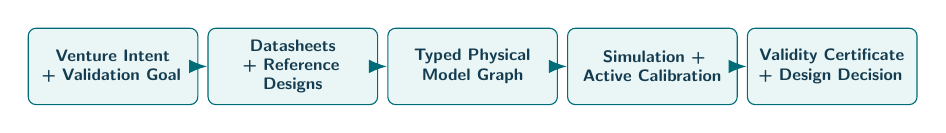
\begin{tikzpicture}[
 node distance=1.15mm,
 box/.style={draw=VMTeal,rounded corners=1mm,fill=VMLight,align=center,minimum height=9.7mm,text width=19.2mm,font=\fontsize{6.35}{7.0}\selectfont\bfseries,text=VMDark},
 arrow/.style={-Latex,thick,color=VMTeal}
]
\node[box] (a) {Venture Intent\\+ Validation Goal};
\node[box,right=of a] (b) {Datasheets\\+ Reference Designs};
\node[box,right=of b] (c) {Typed Physical\\Model Graph};
\node[box,right=of c] (d) {Simulation +\\Active Calibration};
\node[box,right=of d] (e) {Validity Certificate\\+ Design Decision};
\draw[arrow] (a)--(b); \draw[arrow] (b)--(c); \draw[arrow] (c)--(d); \draw[arrow] (d)--(e);
\end{tikzpicture}

\vspace{1.2mm}
\begin{minipage}{0.97\linewidth}
\begin{itemize}
\item \textbf{Grounded compilation:} extract requirements, units, operating ranges, interfaces, validity conditions, calibration relationships, and provenance.
\item \textbf{Constrained synthesis:} select and instantiate validated primitives for sensing, sampling, noise, communication, power, and low-voltage actuation instead of freely inventing equations.
\item \textbf{Hybrid modeling:} combine first-principles models with compact residual models for bias, noise, delay, and component variation not captured in datasheets.
\item \textbf{Active calibration:} recommend the smallest safe physical-test sequence expected to reduce uncertainty and separate confounded error sources.
\item \textbf{Validity certification:} report calibrated intervals, supported operating regions, unresolved assumptions, and out-of-domain refusal conditions.
\end{itemize}
\end{minipage}

\vspace{0.8mm}
\colorbox{VMLight}{\parbox{0.94\linewidth}{\centering\textbf{Phase I technical wedge:} ESP32-S3 connected sensing, Wi-Fi, curated sensors, and simple low-voltage actuation.}}
\end{vmBox}
\end{minipage}
\hfill
\begin{minipage}[t]{0.215\textwidth}
\begin{vmBox}[height=34mm]{Phase I Objectives and Measures}
\textbf{Objectives}
\begin{enumerate}
\item Provenance-linked model compiler
\item Hybrid modeling + active calibration
\item Sim-to-real validity certification
\end{enumerate}

\textbf{Measures}
\begin{itemize}
\item Executability and expert correction
\item Prediction error and UQ coverage
\item Tests required for calibration
\item Fault localization and decision time
\end{itemize}
\end{vmBox}

\vspace{1.7mm}
\begin{vmBox}[height=32mm]{Team and Collaboration Ask}
\textbf{PI:} modeling, simulation, UQ, active experiment design, benchmarking, and R\&D leadership.

\textbf{Altitut:} LLM/datasheet processing, venture workflow, platform integration, and university partnerships.

\textbf{Seeking:} embedded/robotics consultant, university pilots, and collaborators in model-based design and engineering education. An EE/robotics candidate has been identified; participation is pending employer approval.
\end{vmBox}
\end{minipage}

\vspace{1.5mm}

% Prior-art matrix
{\fontsize{8.4}{9.0}\selectfont\bfseries\color{VMDark}Prior-Art Matrix and Working Differentiation}
{\fontsize{6.45}{7.1}\selectfont\color{black!66}\quad Novelty claim to be confirmed through a fuller literature, patent, and commercial-product review.}

\vspace{0.7mm}
\renewcommand{\arraystretch}{1.04}
\setlength{\tabcolsep}{1.75pt}
\fontsize{5.85}{6.55}\selectfont
\begin{tabularx}{\textwidth}{>{\raggedright\arraybackslash}p{23mm} >{\raggedright\arraybackslash}p{43mm} c c c c >{\raggedright\arraybackslash}X}
\toprule
\rowcolor{VMDark}
\color{white}\textbf{Approach} & \color{white}\textbf{Primary contribution} & \color{white}\textbf{Intent} & \color{white}\textbf{Datasheet} & \color{white}\textbf{Active cal.} & \color{white}\textbf{Validity/UQ} & \color{white}\textbf{Boundary relative to VentureMath} \\
\midrule
\textbf{ModiGen}\source{https://arxiv.org/abs/2503.18460}{1} & Modelica component and test-case generation using fine-tuning, graph RAG, and feedback optimization. & \no & \no & \no & \no & Improves simulation-code generation; does not start from venture requirements or certify a model against physical measurements. \\
\rowcolor{VMGray}
\textbf{SimuAgent}\source{https://openreview.net/forum?id=mMB3Y1ERqi}{2} & Simulink agent with compact representation, plan--execute workflow, reflection-guided RL, and SimuBench evaluation. & \partmark & \no & \no & \no & Automates model construction and analysis inside an existing environment; no manufacturer-evidence grounding or sim-to-real validity claim. \\
\textbf{D2S-FLOW}\source{https://arxiv.org/abs/2502.16540}{3} & LLM extraction of electrical parameters from datasheets to generate SPICE device models. & \no & \yes & \no & \no & Strong component-level precedent; no heterogeneous system composition, minimal-test calibration, or system-level validity certificate. \\
\rowcolor{VMGray}
\textbf{Uncertainty-aware twins}\source{https://arxiv.org/abs/2501.10337}{4}\source{https://arxiv.org/abs/2507.01047}{5} & UQ, robust control, active learning, or online updating for an already specified twin or surrogate. & \no & \no & \yes & \yes & Addresses uncertainty after a twin is defined; generally assumes expert-selected scope, variables, and data pipeline. \\
\textbf{VentureMath (proposed)} & Compile venture goal and component evidence into a typed minimum-viable twin, then perform sparse calibration and explicit validity certification. & \yes & \yes & \yes & \yes & Intended differentiator: jointly solve model creation, evidence grounding, cross-component composition, sparse physical calibration, and trustworthy decision boundaries for non-expert venture teams. \\
\bottomrule
\end{tabularx}

\vspace{1.0mm}
\fontsize{6.45}{7.2}\selectfont
\begin{minipage}[t]{0.62\textwidth}
\colorbox{VMLight}{\parbox{0.985\linewidth}{
\textbf{Immediate validation plan:}
(1) interview 5--10 university entrepreneurship and makerspace leaders; 
(2) define 10--15 component primitives, 8--12 venture tasks, three physical prototypes, and controlled faults/non-idealities; 
(3) compare with unconstrained LLM generation, static templates, and expert models; 
(4) complete patent/product prior-art review; 
(5) formalize an embedded-systems consultant and pilot partners.
}}
\end{minipage}
\hfill
\begin{minipage}[t]{0.365\textwidth}
{\fontsize{5.35}{6.0}\selectfont\color{black!72}
\textbf{Representative sources.}
[1] Xiang et al., ``ModiGen,'' 2025.
[2] Liang and Zhao, ``SimuAgent,'' OpenReview/ICLR 2026 submission.
[3] Chen et al., ``D2S-FLOW,'' 2025.
[4] Chen et al., ``Uncertainty-Aware Digital Twins,'' 2025.
[5] Burnett et al., ``Variational Digital Twins,'' 2025.
}
\end{minipage}

\end{document}
